\documentclass{article}
\usepackage{array}
\usepackage{graphicx}
\setlength\parindent{0pt}
\usepackage[obeyspaces]{url}

\title{Setting up GenAMap}
\author{}
\date{}

\begin{document}

\maketitle


In this tutorial, we describe how to you can download and set up GenAMap to run on your machine. For questions / feedback / suggestions, please contact \url{genamapsupport@cs.cmu.edu}.\\

The GenAMap software can be downloaded from this website: \url{http://sailing.cs.cmu.edu/genamap/join.html}. Please click on the link as shown in Figure \ref{downloadButton}. This will start the download of a zipped folder with name `GenAMap\textless version code\textgreater'. Once the download as finished, unzip this folder and move the result to a location of your choice. We call this folder the {\it GenAMap folder}. Please ensure that enough free disk space is available in that location, as GenAMap will use it to store the data you import into the software or create within it.\\

There is no installation procedure for GenAMap. GenAMap can be started directly from the GenAMap folder and will only ever write information to that folder. To run GenAMap, you need to have Java version 6 or newer installed. If you do not currently have Java 6 or newer installed, please download it from here: \url{http://java.com/en/download/index.jsp}.\\

Starting GenAMap will only work when you are connected to the internet. Furthermore, if you are connecting from outside CMU, you will first need to have your IP address manually authenticated to access our web server. For this purpose, please email your IP address to \url{genamapsupport@cs.cmu.edu}. You can determine your IP address, for example, by typing ``IP address'' into Google.\\

There are several ways to start GenAMap. The quick way is to execute \url{_runGenAMap.sh} (Linux) or \url{_runGenAMap.bat} (Windows) in the GenAMap folder, for example by double-clicking on it, or to double-click directly on the GenAMap executable \url{GenAMapMain.jar} (Windows / Mac). This method may not work if your system is not setup in a certain way. The other way to start GenAMap if to bring up a terminal / command line, navigate to the GenAMap folder and type \url{$(JAVAPATH) -jar -Xmx1024m GenAMapMain.jar}. Here, \url{$(JAVAPATH)} stands for the location of your java executable (e.g. in Windows: \url{C:\Program Files (x86)\Java\jre6\bin\java.exe}). If you are unable to start GenAMap from the command line, please email \url{genamapsupport@cs.cmu.edu}, including any error messages that you receive in the terminal / command line window. If your IP address has not yet been manually authenticated by us, please also include it in your email.\\

When GenAMap starts, you should see a login screen as in Figure \ref{loginScreen}. The next step is to create a user account. GenAMap user accounts are organized by teams. A team is a meta-account that contains multiple user accounts who all share access to the same data. As a new user, you must associate yourself with a team. Do this by either creating a new team or joining a team that one of your collaborators has created. To create a new team, please click on ``New Team''. You will be asked to enter a security code. Please enter X76;;PP!@zxiw. Then, choose a name and passcode for your team. Please remember this name and passcode as it will be needed later.\\

Once you have a team to associate yourself to (either because you just created one or you or your collaborators have created one earlier), it is time to create a user account. Please fill out all the contents of the form on the right hand side and tick the two boxes below. The fields ``User Name'' and ``Password'' contain the information that will be used later to log in. Also, choose your team from the blue dropdown menu. In the field ``security code'', please enter TX12IUM-5PPQ. Then, click on ``Create Account''. You need to provide the passcode for the team (which was assigned when the team was created).\\

Finally, once the user account is created, log in on the left hand side with the credentials that you just chose. This completes the set-up process. You should now see the GenAMap main screen as in Figure \ref{initialScreen}.\\

When you close GenAMap, your login credentials are saved in a file inside the GenAMap folder. When you restart the software, you will be logged in automatically and do not have to re-enter your credentials. Note that you still have to be connected to the internet for GenAMap to be able to log in with those credentials. You can also log out of the software to prevent your credentials from being saved or to log in under a different account. To do this, click the menu called `User' in the top left of the screen and select `Logout'.\\

If you are an Ubuntu user, you can create a desktop icon for GenAMap by opening the file `UbuntuDesktopFile.txt' in the GenAMap folder. Replace the paths in the fields `Exec' and `Icon' with the actual paths of the GenAMap executable and logo in your system. Then rename the file to `UbuntuDesktopFile.desktop' and drag it into the launcher sidebar.

\pagebreak
\clearpage

\begin{figure}
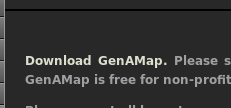
\includegraphics[width=\textwidth]{downloadButton.png}
\caption{Go to http://sailing.cs.cmu.edu/genamap/join.html and click the button shown to download GenAMap}
\label{downloadButton}
\end{figure}

\begin{figure}
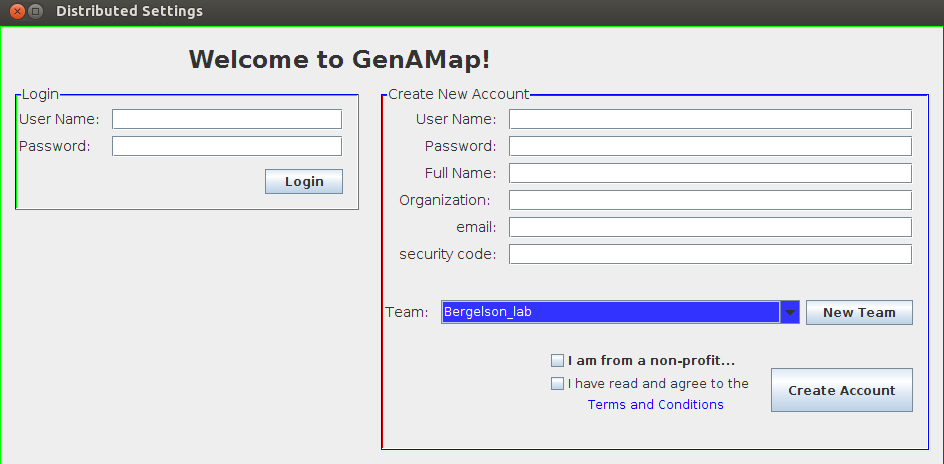
\includegraphics[width=\textwidth]{loginScreen.png}
\caption{GenAMap login screen}
\label{loginScreen}
\end{figure}

\begin{figure}
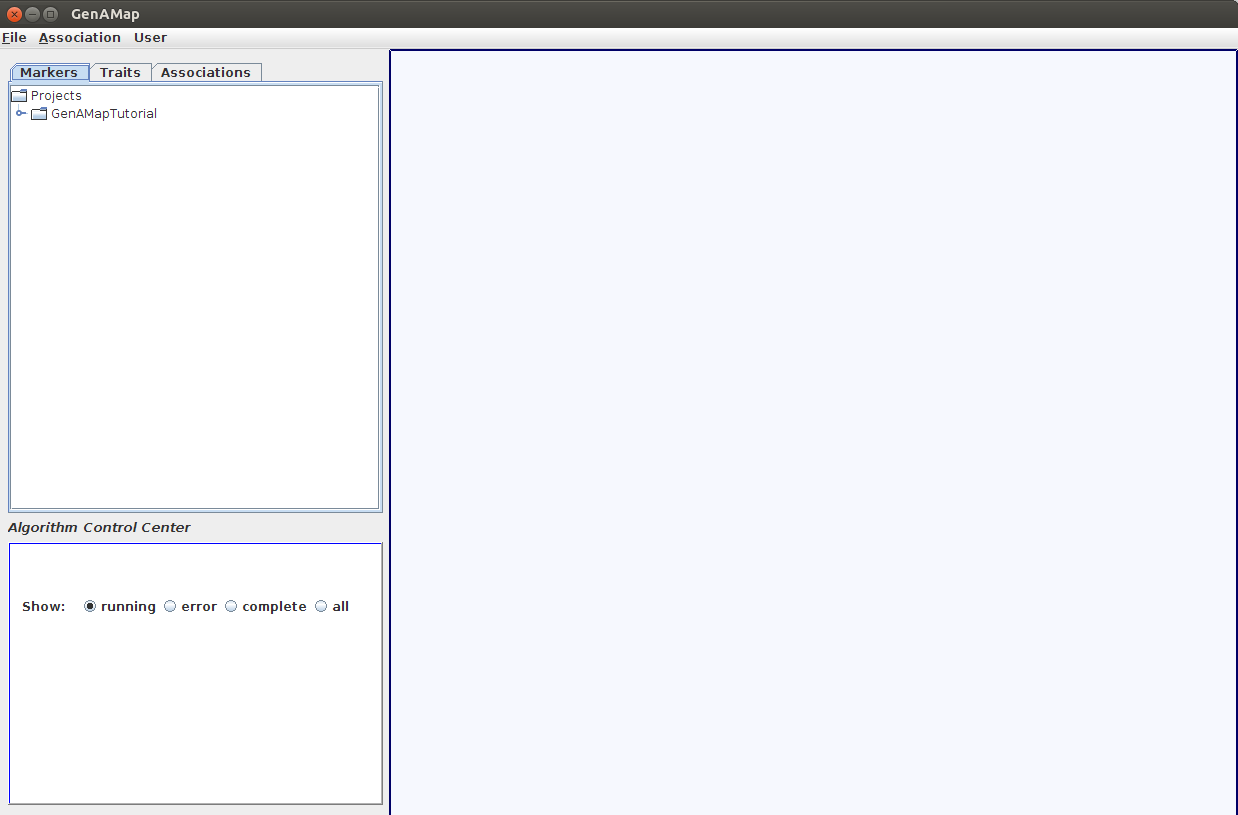
\includegraphics[width=\textwidth]{initialScreen.png}
\caption{GenAMap main screen}
\label{initialScreen}
\end{figure}


\end{document}